\usetikzlibrary{shapes.geometric, arrows.meta, positioning, calc}

\begin{figure}[H]
\centering
\resizebox{0.78\textwidth}{!}{%
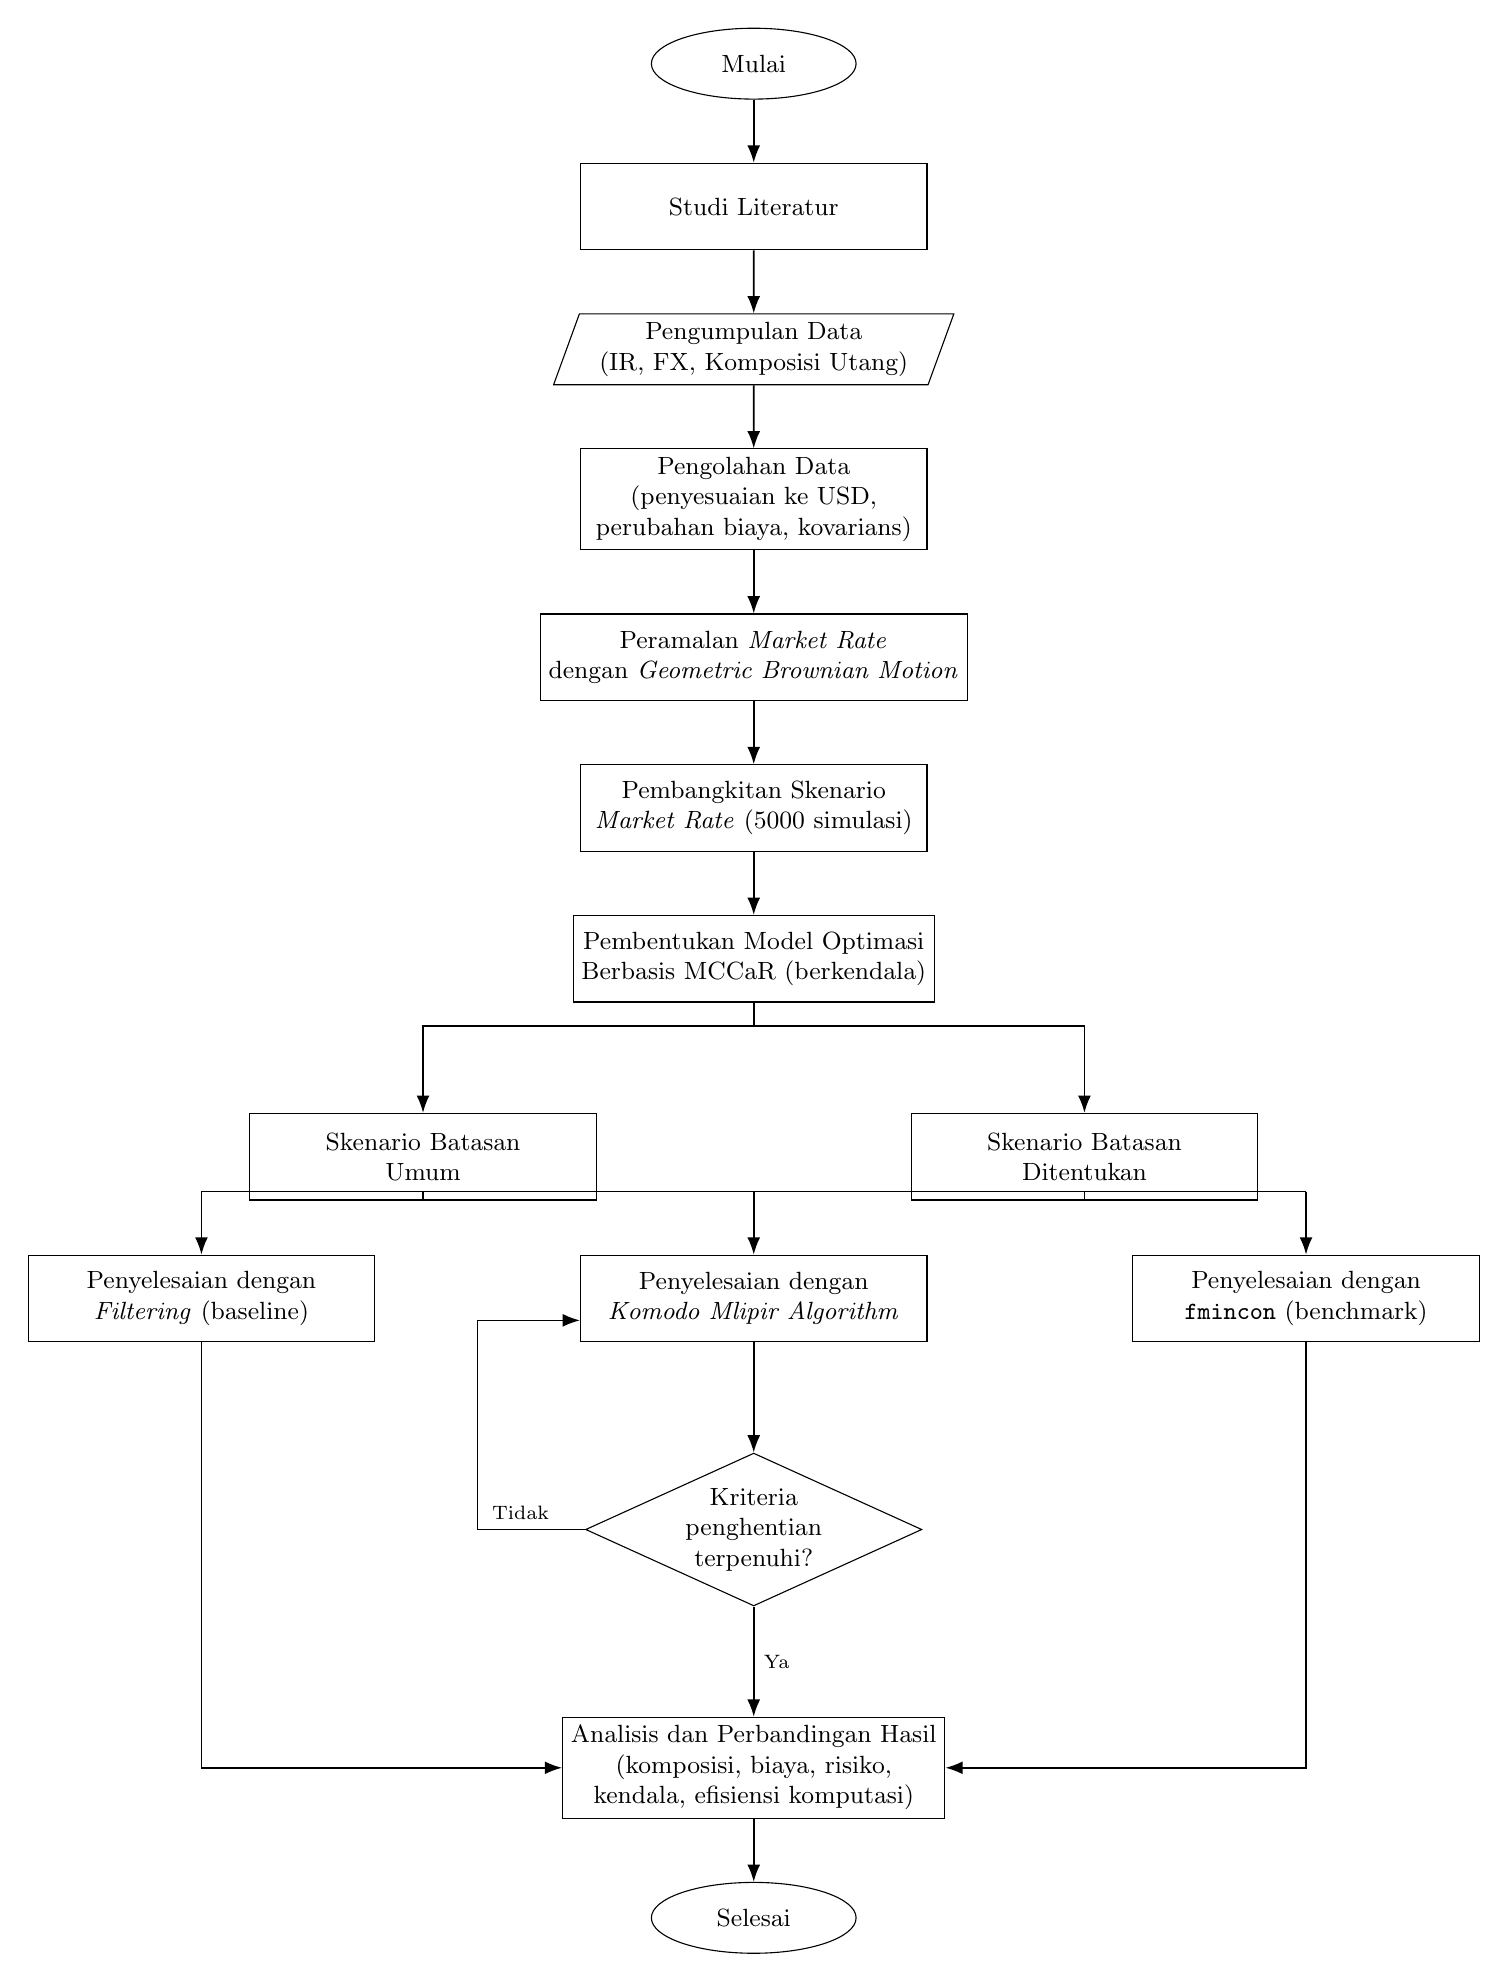
\begin{tikzpicture}[
    node distance = 8mm and 16mm,
    font=\small,
    terminal/.style = {ellipse, draw, minimum width=26mm, minimum height=9mm,
                       align=center, inner sep=2pt},
    io/.style       = {trapezium, draw, trapezium left angle=70,
                       trapezium right angle=110, minimum width=34mm,
                       minimum height=9mm, align=center, inner sep=2pt},
    proc/.style     = {rectangle, draw, minimum width=44mm, minimum height=11mm,
                       align=center, inner sep=3pt},
    decision/.style = {diamond, draw, aspect=2.2, align=center, inner sep=1pt,
                       minimum width=34mm},
    arr/.style      = {-{Latex[length=2.2mm]}, semithick},
    line/.style     = {semithick}
]

% ---- Main spine ----
\node[terminal] (mulai) {Mulai};
\node[proc, below=of mulai] (lit) {Studi Literatur};
\node[io, below=of lit] (input) {Pengumpulan Data\\(IR, FX, Komposisi Utang)};
\node[proc, below=of input] (olah) {Pengolahan Data\\(penyesuaian ke USD,\\perubahan biaya, kovarians)};
\node[proc, below=of olah] (gbm) {Peramalan \textit{Market Rate}\\dengan \textit{Geometric Brownian Motion}};
\node[proc, below=of gbm] (skenario) {Pembangkitan Skenario\\\textit{Market Rate} (5000 simulasi)};
\node[proc, below=of skenario] (model) {Pembentukan Model Optimasi\\Berbasis MCCaR (berkendala)};

% ---- Two scenarios ----
\node[proc, below=14mm of model, xshift=-42mm] (umum)  {Skenario Batasan\\Umum};
\node[proc, below=14mm of model, xshift=42mm]  (tentu) {Skenario Batasan\\Ditentukan};

% ---- Three solvers (placed clearly below the scenario row) ----
\node[proc, below=32mm of model] (kma) {Penyelesaian dengan\\\textit{Komodo Mlipir Algorithm}};
\node[proc, left=of kma, xshift=-10mm]  (filter)  {Penyelesaian dengan\\\textit{Filtering} (baseline)};
\node[proc, right=of kma, xshift=10mm] (fmincon) {Penyelesaian dengan\\\texttt{fmincon} (benchmark)};

% ---- Convergence + analysis + end ----
\node[decision, below=14mm of kma] (konv) {Kriteria\\penghentian\\terpenuhi?};
\node[proc, below=14mm of konv] (analisis) {Analisis dan Perbandingan Hasil\\(komposisi, biaya, risiko,\\kendala, efisiensi komputasi)};
\node[terminal, below=of analisis] (selesai) {Selesai};

% ---- Arrows: spine ----
\draw[arr] (mulai) -- (lit);
\draw[arr] (lit) -- (input);
\draw[arr] (input) -- (olah);
\draw[arr] (olah) -- (gbm);
\draw[arr] (gbm) -- (skenario);
\draw[arr] (skenario) -- (model);

% model -> scenarios
\draw[arr] (model.south) -- ++(0,-3mm) -| (umum.north);
\draw[arr] (model.south) -- ++(0,-3mm) -| (tentu.north);

% scenarios -> solver bus (clean: drop below scenarios, single horizontal bus, then into each solver)
\coordinate (busY) at ($(kma.north)+(0,8mm)$);
\draw[line] (umum.south)  -- (umum.south  |- busY);
\draw[line] (tentu.south) -- (tentu.south |- busY);
\draw[line] (filter.north  |- busY) -- (fmincon.north |- busY);  % horizontal bus spanning all solvers
\draw[arr] (filter.north  |- busY) -- (filter.north);
\draw[arr] (kma.north     |- busY) -- (kma.north);
\draw[arr] (fmincon.north |- busY) -- (fmincon.north);

% KMA -> convergence
\draw[arr] (kma) -- (konv);

% "Tidak" loop: decision west -> up through the clear gap -> into KMA bottom-left
\coordinate (loopX) at ($(filter.east)!0.5!(kma.west)$);
\draw[arr] (konv.west) -- node[above,font=\scriptsize,pos=0.6]{Tidak} (loopX |- konv)
           |- ($(kma.south west)!0.5!(kma.west)$);

% "Ya" -> analysis
\draw[arr] (konv.south) -- node[right,font=\scriptsize]{Ya} (analisis.north);

% filter & fmincon -> analysis (enter left/right edges, not overlapping)
\draw[arr] (filter.south)  |- (analisis.west);
\draw[arr] (fmincon.south) |- (analisis.east);

% analysis -> end
\draw[arr] (analisis) -- (selesai);

\end{tikzpicture}%
}
\caption{Diagram Alir Penelitian}
\label{fig:flowchart-mccar}
\end{figure}
